\section{EAST-WEST asymmetry}\label{section:star_eastWest}
%Since some data-driven corrections are used and they can not be directly validated by closure tests for MC, other tests were performed to check the~correction procedures for data. 
Another kind of consistency check can be performed by comparing the~results obtained by tagging forward-scattered protons in different detectors.
Therefore, each distribution was measured separately for events in which forward-scattered proton
is on one and the other side of the IP (east-west). 
Figure~\ref{fig:eastWest_star} shows the~tests of multiplicity, transverse momentum and pseudorapidity distributions for three ranges of $\xi$, separately. Both statistical uncertainty components, due to input data and due to unfolding matrix, are added in quadrature for $n_\textrm{ch}$ distributions.
The~largest difference is observed for charged-particle multiplicity distributions, where it varies up to $20\%$ for $n_\textrm{ch}=8$ and $0.02 < \xi < 0.1$. 
For the~rest multiplicities and $\xi$ ranges, the~differences are smaller ($<10\%$). In case of $p_\textrm{T}$ and $\bar{\eta}$ distributions, a level of  these disagreements is  below $5\%$. As a~result,
half of the~differences between east and west distributions were used to be  systematic uncertainty.

\begin{comment}
In order to  validate the correction procedures, 
closure tests were performed , i.e. full correction procedure was applied to the MC detector-level distributions and the~results were directly compared to the~true-level distributions. Figure~\ref{fig:closure_star} shows closure tests of multiplicity, transverse momentum and pseudorapidity distributions for three ranges of $\xi$, separately.  PYTHIA~8 SD embedding \ac{MC} was used as an~input. In order  to compare  corrected and true-level distributions, the~statistical uncertainties of the~true-level distributions were assumed to be $0$. Due to the method of factorization of the~global efficiency into the product of single-particle efficiencies, a level of non-closure below $5\%$ is typically considered to be sufficient for the validation of the~procedure. However, the~difference between true-level and corrected distributions was taken as a systematic uncertainties.
\end{comment}
\begin{figure}[h!]
	\centering
	%\vspace{-2.5cm}
	\begin{subfigure}{.49\textwidth}
		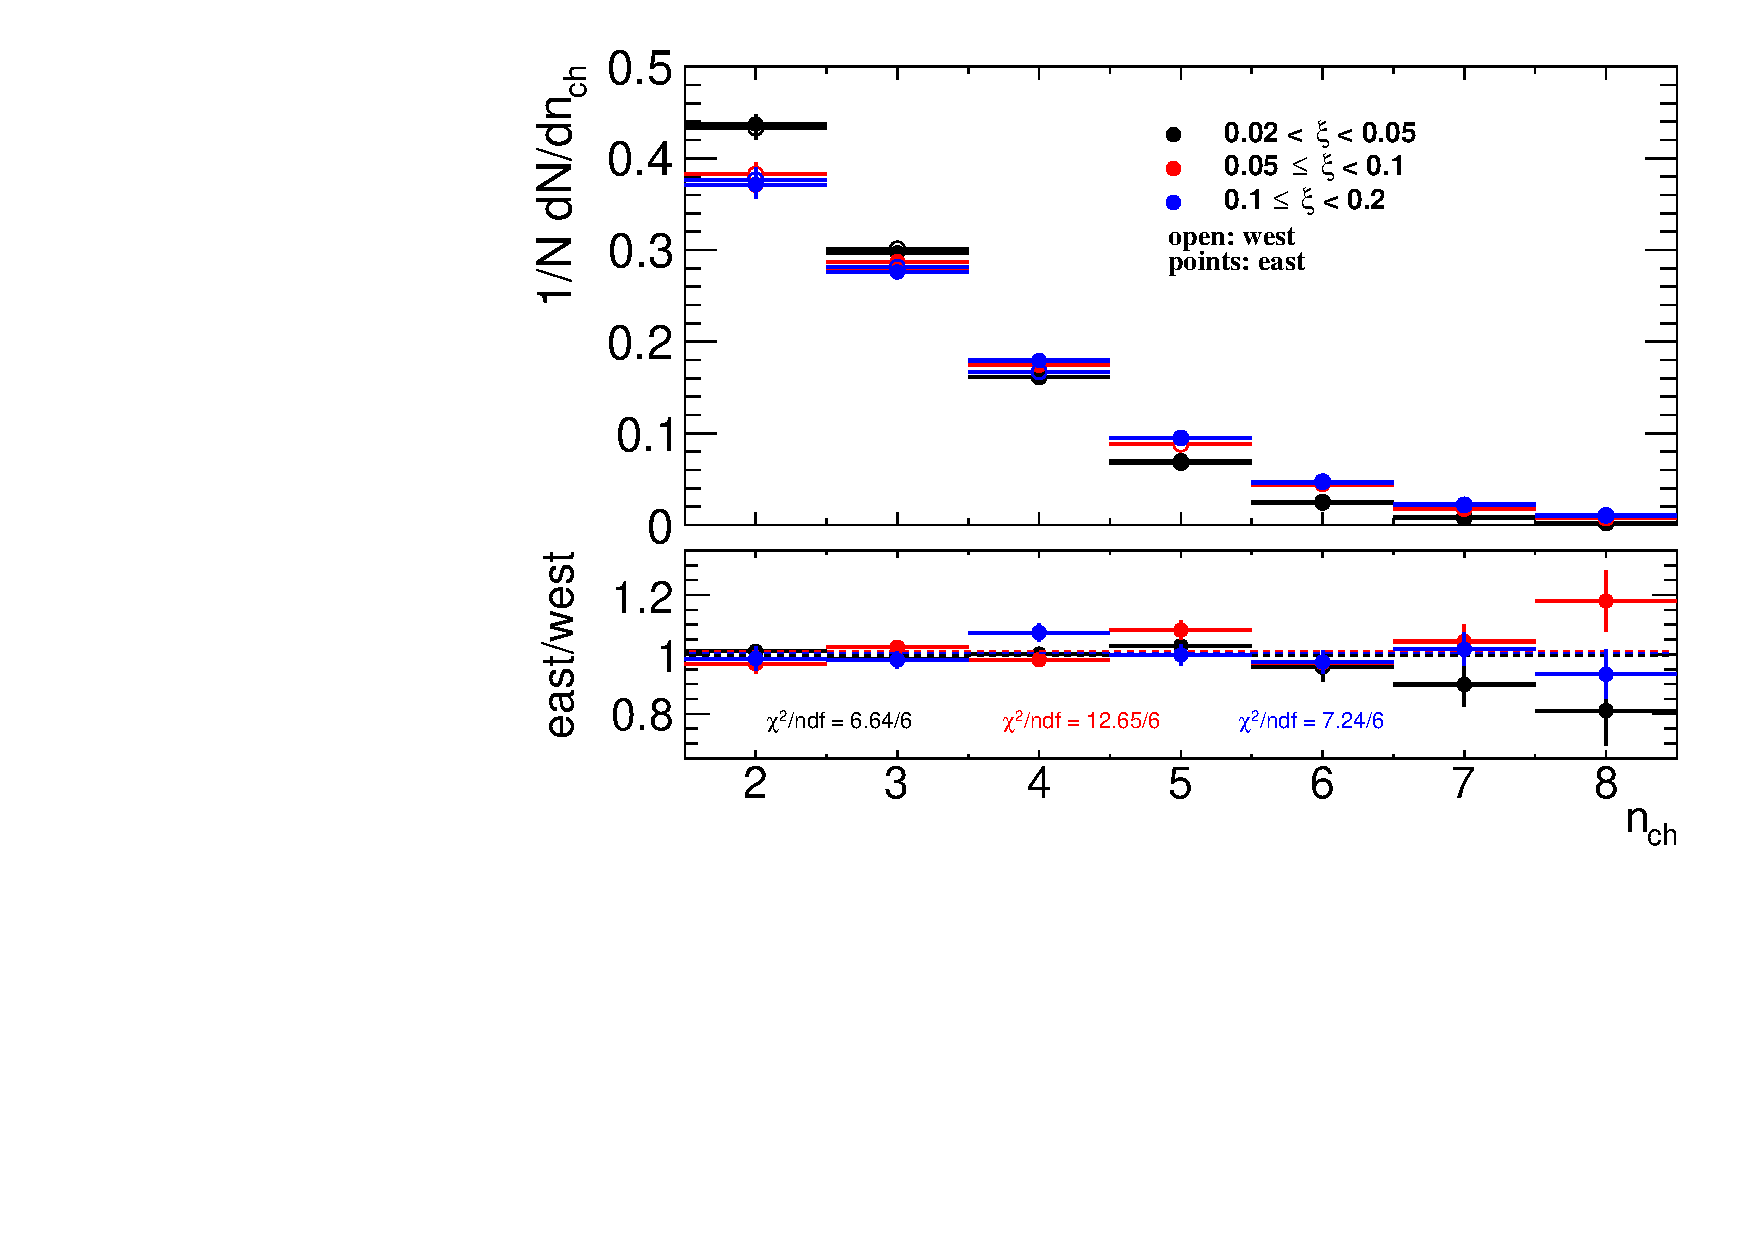
\includegraphics[width=\textwidth,page=1]{chapters/chrgSTAR/img/eastWest/nch_test.pdf}
	\end{subfigure}
	\begin{subfigure}{.49\textwidth}
		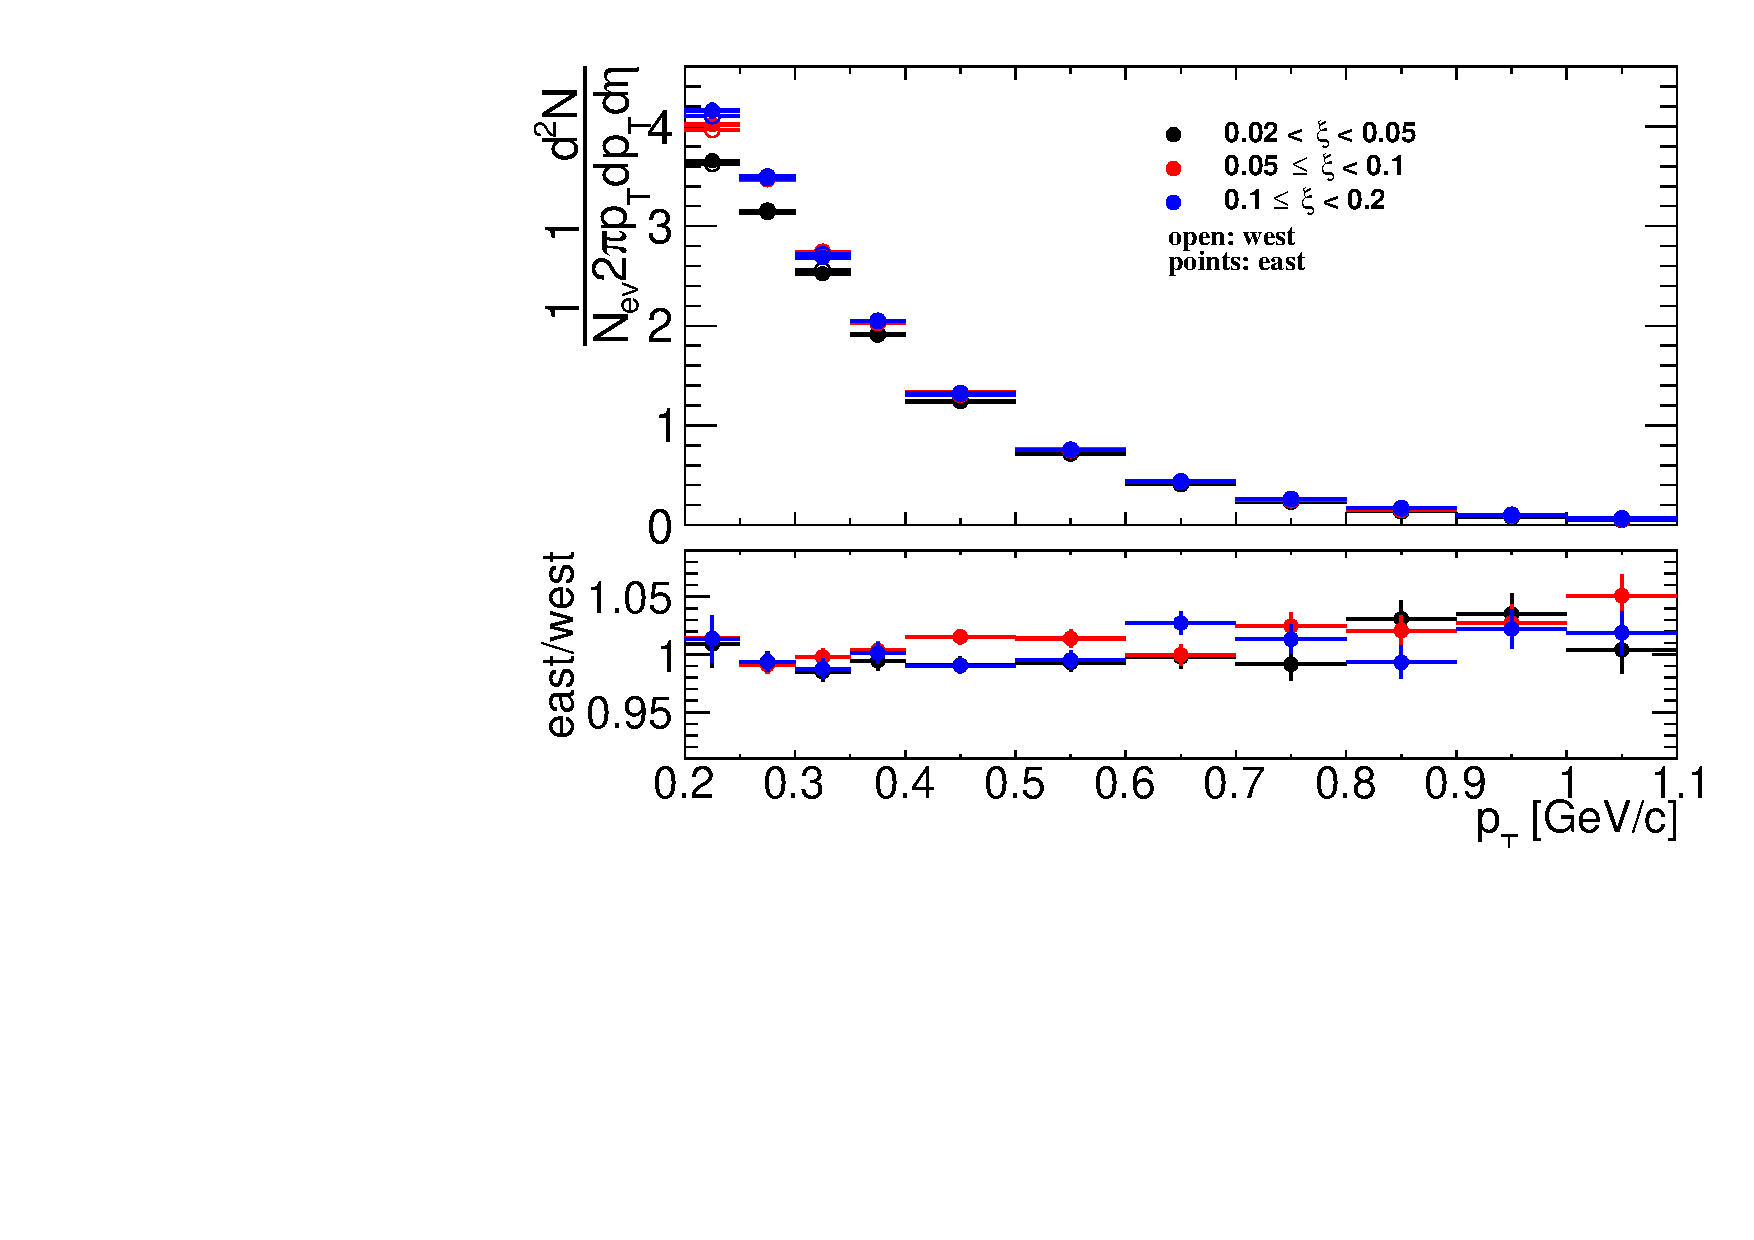
\includegraphics[width=\textwidth,page=1]{chapters/chrgSTAR/img/eastWest/pt_test.pdf}
	\end{subfigure}
	\begin{subfigure}{.49\textwidth}
		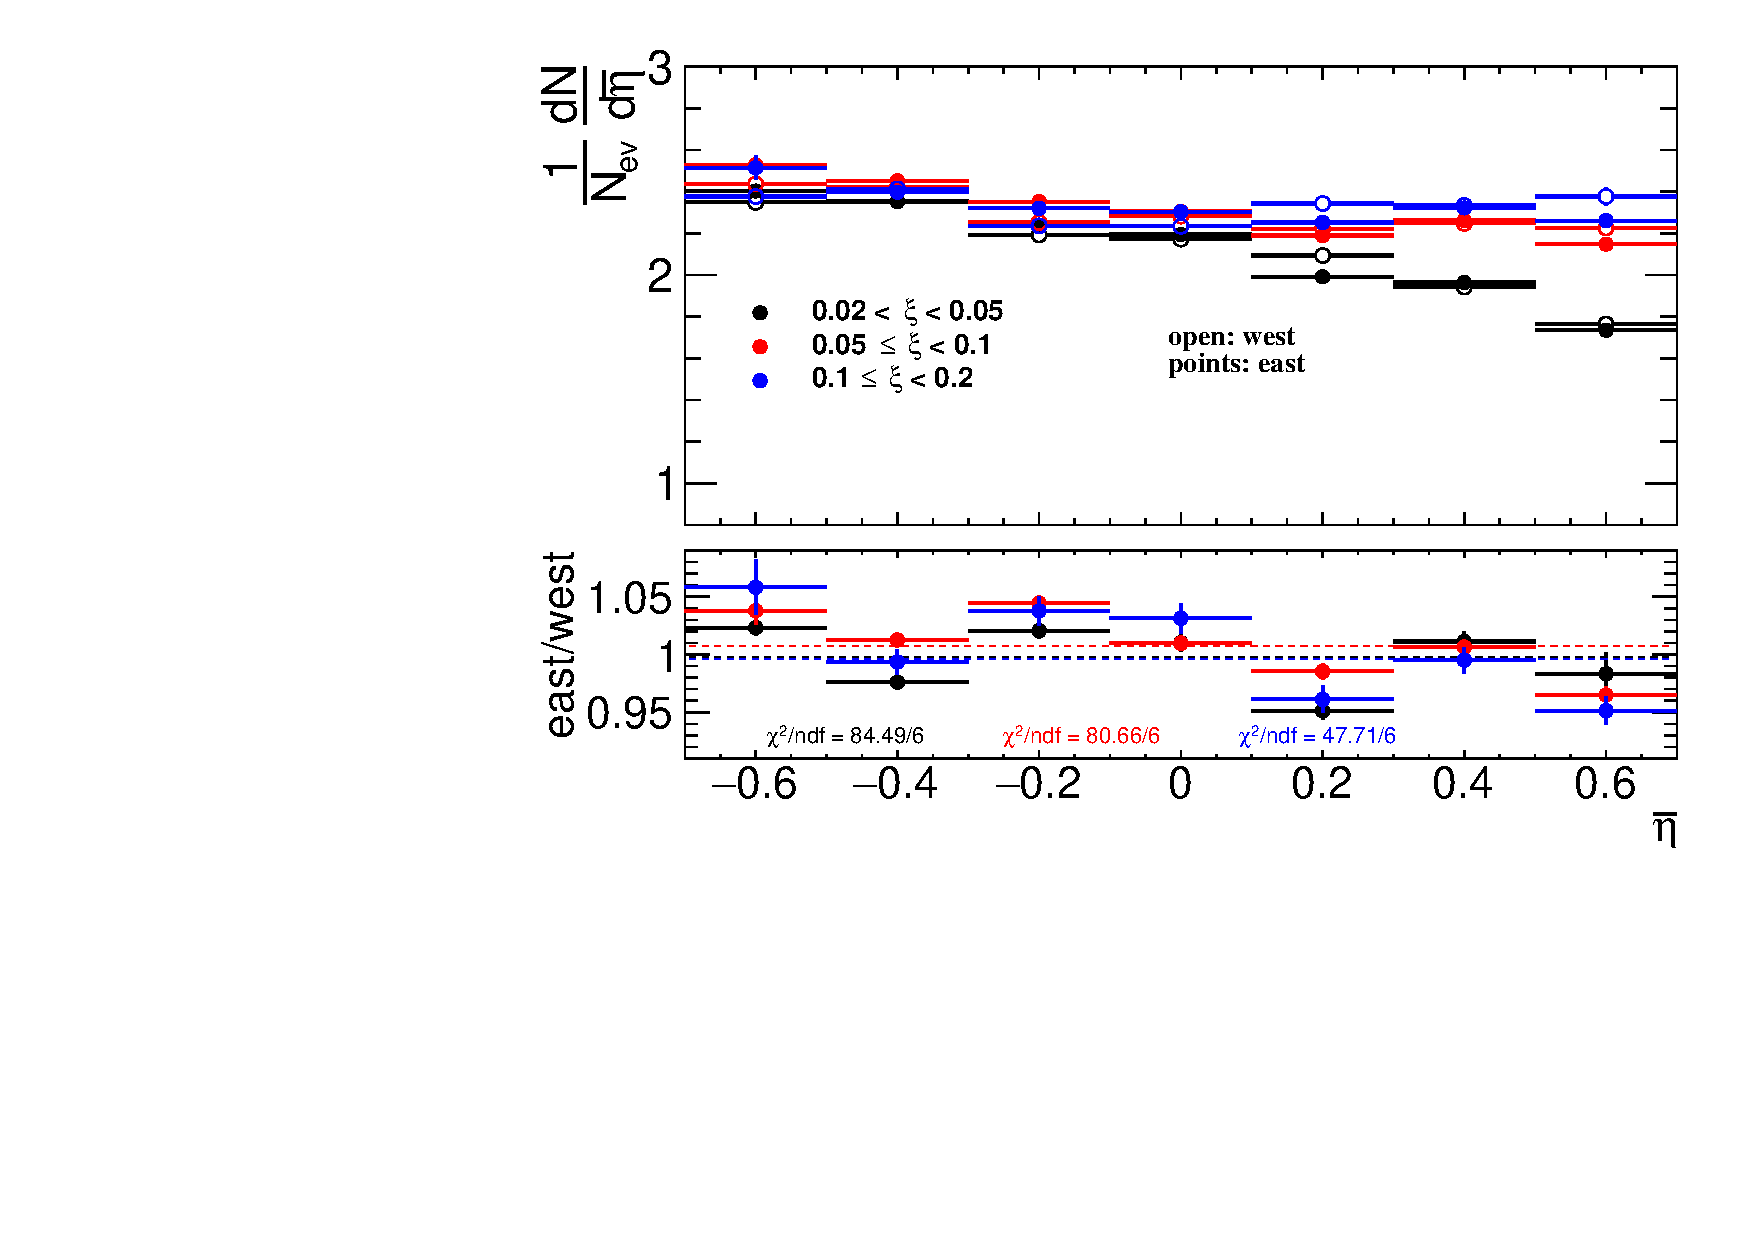
\includegraphics[width=\textwidth,page=1]{chapters/chrgSTAR/img/eastWest/eta_test.pdf}
	\end{subfigure}
	\begin{minipage}{.49\textwidth}
		\caption{(top left) Primary charged-particle multiplicity, (top right) transverse momentum and (bottom) psuedorapidity distributions for three ranges of $\xi$. Particle densities are presented separately for events with forward scattered protons on (open circles) WEST and (full circles) EAST side of the IP. Both statistical uncertainty components, due to input data and due to unfolding matrix, are added in quadrature for $n_\textrm{ch}$ distributions.}
		\label{fig:eastWest_star}
	\end{minipage}
	
	%\vspace{-1.5cm}
	%\vspace{-2cm}
\end{figure}